%=============================================================
\chapter{The Transformation Sub-Model}
\label{chap:transformation}
%=============================================================

\section{Role in the Kinematic Chain}

The \texttt{Transformation} sub-model is a \emph{signal-only} block that computes the cumulative homogeneous transformation from the previous frame $i-1$ to the current frame $i$. 

The transformation chain, as depicted in Figure \ref{fig:transformation_chain}, computes the total transformation with respect to the base frame, while also providing useful intermediate transformations.

\begin{figure}[H]
  \centering
  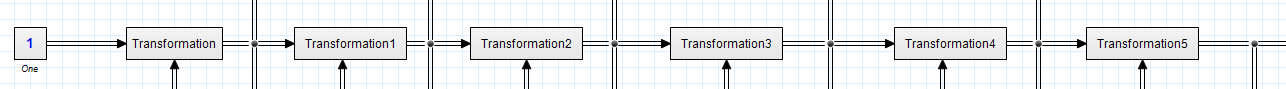
\includegraphics[width=1.0\textwidth]{chapter_transformation/figs/transformation_chain.png}
  \caption{Chain of transformations}
  \label{fig:transformation_chain}
\end{figure}

\section{Ports \& Parameters}
The \texttt{Transformation} sub-model's port structure is as follows:

\begin{center}
\begin{tikzpicture}[
    >=Stealth,
    every node/.style={font=\small},
    line width=0.8pt
]

\def\boxW{4.5}    % width of the black box
\def\boxH{2.2}    % height of the box
\def\arrowLen{2}  % length of arrows

\draw[fill=white, draw=black, line width=1.2pt]
    (0, -\boxH/2) rectangle (\boxW, \boxH/2);

\node[anchor=north, font=\normalsize\bfseries] at (\boxW/2, \boxH/2 - 0.2)
    {Transformation};

\draw[black, line width=0.5pt]
    (0.15, \boxH/2 - 0.7) -- (\boxW - 0.15, \boxH/2 - 0.7);

% DH Parameters
\node[anchor=north, font=\footnotesize, align=center] at (\boxW/2, \boxH/2 - 0.9)
    {$p_\text{body,i}$};

\def\yCentral{0}

% --- Input Signal Arrow (Left) ---
\draw[->, line width=1pt]
    (-\arrowLen, \yCentral) -- (0, \yCentral);
\node[above, font=\small] at (-\arrowLen/2, \yCentral + 0.05) {$\prescript{0}{}{T}_{i-1}$};

% --- Input Signal Arrow (Bottom) ---
\def\xBot{\boxW/2}
\draw[->, line width=1pt]
    (\xBot, -\boxH/2 - 1.5) -- (\xBot, -\boxH/2);
\node[right, font=\small] at (\xBot, -\boxH/2 - 0.75) {$\prescript{i-1}{}{T}_i$};

% --- Output Signal Arrow (Right) ---
\draw[->, line width=1pt]
    (\boxW, \yCentral) -- (\boxW + \arrowLen, \yCentral);
\node[above, font=\small] at (\boxW + \arrowLen/2, \yCentral + 0.05) {$\prescript{0}{}{T}_i$};

\end{tikzpicture}
\end{center}

The only given parameter is the position of the stl body with respect to the DH frame, denoted as $p_{\text{body}, i}$, which is used to offset the link body in the 3D visualization. The corresponding stl orientation is defined inside the \texttt{transformation} block.

\section{Equations}

Given the absolute transformation $\prescript{0}{}{T}_{i-1}$ up to frame $i-1$ and the incremental DH transformation $\prescript{i-1}{}{T}_i$ provided by the \texttt{Joint} block, the absolute transformation is updated as:
\begin{equation}
  \prescript{0}{}{T}_i = \prescript{0}{}{T}_{i-1} \cdot \prescript{i-1}{}{T}_i
  \label{eq:chain}
\end{equation}

The transformation from a general frame $i$ to the base frame is given by the product of the sequential transformations:
$$
\prescript{0}{}{T}_i = \prescript{0}{}{T}_1 \cdot \prescript{1}{}{T}_2 \dots \prescript{i-1}{}{T}_i 
$$

Furthermore, within each transformation block, the following variables are computed:

\begin{itemize}
  \item \textbf{Position of the DH frame with respect to the base frame:} $\prescript{0}{}{p}_i = T[1:3, 4]$, which is utilized to define the position of the DH frames in the 3D visualization. 
  \item \textbf{Orientation of the DH frame with respect to the base frame:} $\prescript{0}{}{R}_i = T[1:3, 1:3]$. This rotation matrix dictates the orientation of the DH frame in the 3D visualization and is also transposed to re-orient the gravity vector from the base frame to the DH frame within the \textbf{MSe} element of the \texttt{Link} block.
  \item \textbf{Position of a relative point on link $i$ with respect to the base frame:} $\prescript{0}{}{p}_{\text{body}, i} = \prescript{0}{}{R}_i \prescript{i}{}{p}_{\text{body}, i} + \prescript{0}{}{p}_i$, used to offset the link body inside the 3D visualization.
  \item \textbf{Orientation of link $i$ with respect to the base frame:} $\prescript{0}{}{R}_{\text{body}, i} = \prescript{0}{}{R}_i \prescript{i}{}{R}_{\text{body}, i}$, used to properly orient the link body in the 3D visualization.
\end{itemize}

Lastly, the complete transformation matrix $T_{\text{next}}$ is utilized inside the gravity compensation block to compute the directional axes $z_i$, the positions of the DH frames $p_i$, and the centers of mass $p_{\text{com}, i}$, all evaluated with respect to the base frame.